%%%% 補助スライド
\appendix
\backupbegin

\begin{frame}{~}
 \centering
 - 補足用 -
\end{frame} 

%%%%%%%%%%%%%%%%%%%%%%%%%%%%%%%%%%%%%%%%%%%%%%%%%%
%% 実験結果
%%%%%%%%%%%%%%%%%%%%%%%%%%%%%%%%%%%%%%%%%%%%%%%%%%
\begin{frame}\frametitle{実験結果: 考察}

  \begin{itemize}
    \item \code{unchanged}符号化は,\code{changed}符号化と比べて有効性を示した.
    \item 要因として,\alert{基礎化後のルール数の差}が考えられる.
    \begin{itemize}
      \item \textit{clingo}では与えられた論理プログラムを充足可能性判定問題へと変換して解く.
      \item ルール数を少なくすることは,節数を少なくすることにつながる.
      \item 節数が多い時,単位伝播やヒューリスティックによる変数選択時のオーバーヘッドが増加する.
      \item ルール数を抑えることでオーバーヘッドの減少につながり,優位性を示したと考えられる.
    \end{itemize}
  \end{itemize}
  
\end{frame}

%%%%%%%%%%%%%%%%%%%%%%%%%%%%%%%%%%%%%%%%%%%%%%%%%%
%% 基礎化
%%%%%%%%%%%%%%%%%%%%%%%%%%%%%%%%%%%%%%%%%%%%%%%%%%
%\begin{frame}\frametitle{基礎化}
%  
%\end{frame}

%%%%%%%%%%%%%%%%%%%%%%%%%%%%%%%%%%%%%%%%%%%%%%%%%%
%% ASP符号化のルール数
%%%%%%%%%%%%%%%%%%%%%%%%%%%%%%%%%%%%%%%%%%%%%%%%%%
\begin{frame}\frametitle{2つの符号化の基礎化後のルール数}

  \begin{itemize}
    \item 基礎化とは,変数を含む述語論理を変数を含まない命題論理へと変換することである.
    \item 遷移制約に関するルール数のみに着目する.
    \item $|L|$をステップ長$\ell$,$|C|$を色数,$|V|$をグラフ$G$の頂点数とする.
  \end{itemize}

  \begin{exampleblock}{}
    \centering
    \begingroup
\renewcommand{\arraystretch}{1.5}
\begin{tabular}{l|c}\hline
  符号化名 & 基礎化後のルール数(遷移制約) \\ \hline
  origin & $4|T|{|C|\choose 2}^{2}{|V|\choose 2}$ \\ \hline
  changed & $|T|\left(2{|C|\choose 2}|V| + 1\right)$ \\ \hline
  unchanged & $|T|(|CV| + 1)$ \\ \hline
\end{tabular}
\endgroup
  \end{exampleblock}

  \begin{itemize}
    \item 遷移制約の基礎化後のルール数は,遷移回数の選び方の組合せ・
          色の選び方の組合せ・グラフの頂点の選び方の組合せの乗算となる.
  \end{itemize}

\end{frame}

%%%%%%%%%%%%%%%%%%%%%%%%%%%%%%%%%%%%%%%%%%%%%%%%%%
%% 符号化コード
%%%%%%%%%%%%%%%%%%%%%%%%%%%%%%%%%%%%%%%%%%%%%%%%%%
\begin{frame}\frametitle{\code{unchanged}符号化}

  \code{unchanged}符号化は,制約$T$に関する記述が
  \code{changed}符号化と異なる.

  \begin{exampleblock}{}
    \centering
    \lstinputlisting{code/gcrp_cc_unchanged.lp}
  \end{exampleblock}
  
\end{frame}

%%%%%%%%%%%%%%%%%%%%%%%%%%%%%%%%%%%%%%%%%%%%%%%%%%
%% 符号化コード
%%%%%%%%%%%%%%%%%%%%%%%%%%%%%%%%%%%%%%%%%%%%%%%%%%
\begin{frame}[fragile]\frametitle{\code{unchanged}符号化}

  \begin{exampleblock}{}
    \centering
    \lstinputlisting[
      basicstyle=\tiny
    ]{code/gcrp_cc_unchanged.lp}
  \end{exampleblock}

  \begin{onlyenv}<1>
    \begin{exampleblock}{}
      \centering
      \begin{lstlisting}
unchanged(X,T) :- color(X,C,T), color(X,C,T-1), 
                  T >= 1.
      \end{lstlisting}
    \end{exampleblock}
    \begin{itemize}
      \item ステップ数$T-1$とステップ数$T$で頂点$X$の色が変化しなかったことを意味する
            アトム\code{unchanged/2}を導入している.
    \end{itemize}
  \end{onlyenv}

  \begin{onlyenv}<2>
    \begin{exampleblock}{}
      \centering
      \begin{lstlisting}
:- not N-1 { unchanged(X,T) } N-1 , 
    n(N), t(T), T >= 1.
      \end{lstlisting}
    \end{exampleblock}
    \begin{itemize}
      \item 色が変わらない頂点は各遷移において$N-1$個であることを表している.
    \end{itemize}
  \end{onlyenv}
  
\end{frame}

%%%%%%%%%%%%%%%%%%%%%%%%%%%%%%%%%%%%%%%%%%%%%%%%%%
%% k彩色遷移問題
%%%%%%%%%%%%%%%%%%%%%%%%%%%%%%%%%%%%%%%%%%%%%%%%%%
\begin{frame}\frametitle{$k$彩色遷移問題の性質}

  \begin{itemize}
    \item 色数$k$によって問題の性質が異なることが知られている.
    \begin{itemize}
      \item \structure{$k=2$}のとき,グラフGは2部グラフであり\structure{明らかに到達不能}~[Cereceda+ '08].
      \item \structure{$k=3$}のとき,\structure{クラスP}に属する~[Cereceda+ '08].
      \item \structure{$k \ge 4$}のとき,一般に\structure{\textbf{PSPACE完全}}となる~[Bonsma+ '09].
    \end{itemize}

    \item グラフの形に制限を加えることにより,多項式時間で解決可能となるものが存在することがわかっている~[Bonsma+ '09].
    \begin{itemize}
      \item 平面グラフであり,かつ$k \ge 7$のとき.
      \item 2部平面グラフであり,かつ$k \ge 5$のとき.
    \end{itemize}

  \end{itemize}

\end{frame}

%%%%%%%%%%%%%%%%%%%%%%%%%%%%%%%%%%%%%%%%%%%%%%%%%%
%% グラフ点彩色問題
%%%%%%%%%%%%%%%%%%%%%%%%%%%%%%%%%%%%%%%%%%%%%%%%%%
\begin{frame}\frametitle{グラフ点彩色問題}
    
  \begin{block}{グラフ点彩色問題の定義}
    与えられたグラフ$G=(V, E)$と色数$k$に対して,以下の制約を満たす解が存在するかを判定する問題.
    \begin{itemize}
      \item 各頂点は一つの色で塗られる.
      \item $(u, v) \in E$である$u, v \in V$について,$u$と$v$は異なる色で塗られる.
    \end{itemize}
  \end{block}
  
  \begin{exampleblock}{グラフ点彩色問題の例($k=4$)}
    \begin{columns}
      \begin{column}{1.0\textwidth}
        \centering
        %%%%%%%%%%%%%%%%%%%%%%%%%%%%%%%%%%%%%%%%%%%%%%%%%%
% 実行例(t=0) (第6章で使う)
%%%%%%%%%%%%%%%%%%%%%%%%%%%%%%%%%%%%%%%%%%%%%%%%%%

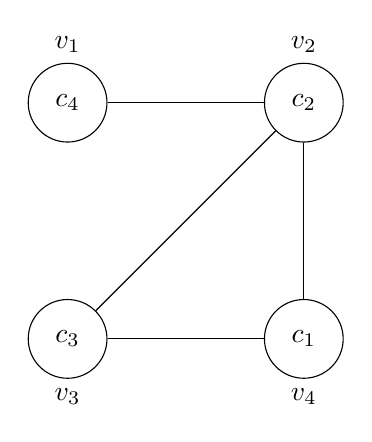
\begin{tikzpicture}[x=1.5cm, y=1.5cm]

  % 設定
  \tikzset{node/.style={circle,draw=black,minimum size=1cm}}
 

 
  % 補助線
  % \draw [help lines,blue] (0,0) grid (20,6);
 
  % node %
  \node[node, label=above:$v_1$] at (-1,1) (node1) {$c_4$};
  \node[node, label=above:$v_2$] at (1,1) (node2) {$c_2$};
  \node[node, label=below:$v_3$] at (-1,-1) (node3) {$c_3$};
  \node[node, label=below:$v_4$] at (1,-1) (node4) {$c_1$};
 
  \foreach \u / \v in {node1/node2, node2/node3, node2/node4, node3/node4}
  \draw (\u) -- (\v);
 \end{tikzpicture}
 
 %%%%%%%%%%%%%%%%%%%%%%%%%%%%%%%%%%%%%%%%%%%%%%%%%%%%%%%%%%
 %%% Local Variables:
 %%% mode: japanese-latex
 %%% TeX-master: paper.tex
 %%% End:
 
      \end{column}
    \end{columns}
  \end{exampleblock}

\end{frame}

%%%%%%%%%%%%%%%%%%%%%%%%%%%%%%%%%%%%%%%%%%%%%%%%%%
%% PSPACE
%%%%%%%%%%%%%%%%%%%%%%%%%%%%%%%%%%%%%%%%%%%%%%%%%%
%\begin{frame}\frametitle{クラスPSPACE}
%
%  \begin{itemize}
%    \item 計算量のクラスの一つ.
%    \item 決定性チューリングマシンに多項式量のメモリを与えることで解決できる問題が属する.
%    \item 指数時間で解くことが可能.
%    \item P$\subseteq$NP$\subseteq$PSPACEであることはわかっている.
%    \begin{itemize}
%      \item ただし, 真に包含するかは未解決.
%    \end{itemize}
%  \end{itemize}
%  
%\end{frame}

\backupend